% This example is meant to be compiled with lualatex or xelatex
% The theme itself also supports pdflatex
\PassOptionsToPackage{unicode}{hyperref}
\documentclass[aspectratio=169, 12pt]{beamer}
\usepackage[german,english]{babel}

% Load packages you need here
\usepackage{polyglossia}
\setmainlanguage{german}

\usepackage{csquotes}

% Tikz plots
\usepackage{pgfplots}
% \DeclareUnicodeCharacter{2212}{−}
\usepgfplotslibrary{groupplots,dateplot}
\usetikzlibrary{patterns,shapes.arrows}
\pgfplotsset{
  compat=newest,
  legend style={
    font=\scriptsize,
  },
  x tick label style={
    font=\scriptsize,
    /pgf/number format/.cd,
    use comma,
    % fixed,
    % fixed zerofill,
    % precision=1,
    /tikz/.cd
  },
  y tick label style={
    font=\scriptsize,
    /pgf/number format/.cd,
    use comma,
    fixed,
    fixed zerofill,
    precision=3,
    scaled ticks=false,
    /tikz/.cd
  },
  x label style={font=\footnotesize},
  y label style={font=\footnotesize}
}

\usepackage{subcaption}
\usepackage{tikz}
\usetikzlibrary{shapes}
\usetikzlibrary{arrows}
\usetikzlibrary{positioning}
\usepackage{tikzscale}
    

\usepackage{amsmath}
\usepackage{amssymb}
\usepackage{mathtools}

\usepackage{hyperref}
\usepackage{bookmark}

\usepackage{graphicx}
\usepackage{wrapfig}

\usepackage[utf8]{inputenc}
% \usepackage{pgfplots}
% % \DeclareUnicodeCharacter{2212}{−}
% \usepgfplotslibrary{groupplots,dateplot}
% \usetikzlibrary{patterns,shapes.arrows}
% \pgfplotsset{
%   compat=newest,
%   legend style={
%     font=\scriptsize,
%   },
%   x tick label style={
%     font=\scriptsize,
%     /pgf/number format/.cd,
%     use comma,
%     % fixed,
%     % fixed zerofill,
%     % precision=1,
%     /tikz/.cd
%   },
%   y tick label style={
%     font=\scriptsize,
%     /pgf/number format/.cd,
%     use comma,
%     fixed,
%     fixed zerofill,
%     precision=1,
%     /tikz/.cd
%   },
%   x label style={font=\footnotesize},
%   y label style={font=\footnotesize}
% }
% \pgfplotsset{compat=newest}

% load the theme after all packages

\usetheme[
  showtotalframes, % show total number of frames in the footline
]{tudo}

\setbeamertemplate{section in toc}[sections numbered]

% Put settings here, like
\unimathsetup{
  math-style=ISO,
  bold-style=ISO,
  nabla=upright,
  partial=upright,
  mathrm=sym,
}
\setmathfont[range={\mathcal,\mathbfcal},StylisticSet=1]{XITS Math}

% Tikz
\usepackage{tikz}
\usetikzlibrary{shapes,arrows}

\DeclareMathOperator{\dct}{dct}
\DeclareMathOperator{\idct}{idct}
\DeclareMathOperator{\dwt}{dwt}
\DeclareMathOperator{\idwt}{idwt}
\DeclareMathOperator{\NSE}{NSE}
\DeclareMathOperator{\acc}{acc}

\title{Kompression neuronaler Netze mit Hilfe von Wavelet Transformationen}
\author[L.~Camphausen]{Lucas Camphausen}
\date{6. September 2022}
\institute[LS 11]{Lehrstuhl für Algorithm Engineering (LS 11) \\  Fakultät für Informatik \\~\\ Betreuer: Prof. Dr. Rudolph, Dr.-Ing. Brehler (Fraunhofer IML)}
% \betreuer{Prof. Dr. Rudolph, Dr. Marius Brehler (Fraunhofer IML)}
% \titlegraphic{\includegraphics[height=4.3cm]{example-image-a}}


\begin{document}

\begin{tiny}
  \maketitle
\end{tiny}

% --- Übersicht
\begin{frame}{Übersicht}
  \tableofcontents
\end{frame}
% --- Übersicht

% === Motivation
\section{Motivation}

\begin{frame}{Übersicht}
  \tableofcontents[currentsection]
\end{frame}

% --- Motivation 1
\begin{frame}{Motivation}
  \begin{itemize}
    \item Convolutional Neural Networks (CNN) sind ein vielfach genutztes Konzept des Maschinellen Lernens.
    \item Speicherbedarf ist verhältnismäßig groß:
          \begin{itemize}
            \item VGG16: 520 MB
            \item ResNet18: 40 MB
            \item MobileNet v2: 16 MB
          \end{itemize}
    \item Ausführung auf ressourcenbeschränkter Hardware problematisch:
          \begin{itemize}
            \item Teils stehen nur wenige MB Flash zur Verfügung.
            \item Ressourcenverbrauch (insb. Speicherbedarf) muss gesenkt werden.
          \end{itemize}
  \end{itemize}
\end{frame}
% --- Motivation 1

% === Motivation

% === Stand der Forschung
\section{Stand der Forschung}

\begin{frame}{Übersicht}
  \tableofcontents[currentsection]
\end{frame}

% --- Stand der Forschung 1
\begin{frame}{Stand der Forschung}
  Verschiedene Techniken zur Kompression stehen zur Verfügung:

  \begin{itemize}
    \item Quantisierung
          \begin{itemize}
            \item Reduzierung des Speicherbedarfs der einzelnen Parameter
            \item Repräsentation der Parameter mit geringerer Genauigkeit (16-bit Gleitkommazahl, 8-bit Ganzzahl, Boolean)
          \end{itemize}
    \item Pruning
          \begin{itemize}
            \item Reduzierung der Anzahl an Parametern
            \item Unstrukturiertes Entfernen einzelner unwichtiger Parameter
            \item Strukturiertes Entfernen von Filtern
          \end{itemize}
  \end{itemize}
\end{frame}
% --- Stand der Forschung 1

% --- Stand der Forschung 2
\begin{frame}{Stand der Forschung}
  \begin{itemize}
    \item Weight-Sharing
          \begin{itemize}
            \item Ausnutzen von Ähnlichkeiten zwischen Filtern
            \item Clustering von Filtern
            \item Speicherung der Clusterzentren
          \end{itemize}
    \item Transformationsbasierte Kompression
          \begin{itemize}
            \item Parallelen zur Kompression von Bilddaten
            \item Transformation der Daten in andere Repräsentation:
                  \begin{itemize}
                    \item JPEG (Diskrete Kosinus Transformation)
                    \item JPEG 2000 (Diskrete Wavelet Transformation)
                  \end{itemize}
            \item Vernachlässigung von unwichtigen Koeffizienten
          \end{itemize}
  \end{itemize}
\end{frame}
% --- Stand der Forschung 2

% === Grundlagen
\section{Transformationsbasierte Kompression}

\begin{frame}{Übersicht}
  \tableofcontents[currentsection]
\end{frame}

% Präteritum
% ggf überarbeiten
\begin{frame}{Ziel der Arbeit}
  Ziel der Arbeit ist die Untersuchung der Möglichkeiten neuronale Netze mit Hilfe der Diskreten Wavelet Transformation zu komprimieren.
  Folgende Aspekte sollen betrachtet werden:
  \begin{itemize}
    \item Wie lässt sich durch die DWT eine Kompression erreichen?
    \item Welche Kompressionsraten können erreicht werden?
    \item Inwiefern verbessert sich die Situation bei der Ausführung auf einem Mikrocontroller?
    %\item Ist es möglich das Netz auf einem Mikrocontroller bare-metal ohne Betriebssystem auszuführen?
    \item Genauigkeit und Laufzeit sind nicht immer die kritischen Messgrößen.
    \item Es soll mit der DCT verglichen werden.
  \end{itemize}
\end{frame}

% --- Grundlagen 1
% \begin{frame}{Grundlagen}
%   Die Gewichte, vor allem die der Faltungsschichten, sollen auf folgende Art komprimiert werden:
%   \begin{itemize}
%     \item Filter werden in Blöcken gruppiert.
%           \begin{itemize}
%             \item Im einfachsten Fall bildet jeder Filter einen eigenen Block.
%           \end{itemize}
%     \item Blöcke werden mit der DWT transformiert.
%     \item Für jedes Subband wird ein Clustering mit verschiedenen Parametern durchgeführt.
%     \item Clusterzentren werden gespeichert.
%     \item Das Netz wird nachtrainiert.
%   \end{itemize}
% \end{frame}
% --- Grundlagen 1

% --- DCT 1
\begin{frame}{Diskrete Kosinus Transformation (DCT)}
  \begin{itemize}
    \item DCT ist eine Transformation aus dem Orts- in den Frequenzbereich.
    \item Eingangssignal wird als Linearkombination von Kosinusfunktionen verschiedener Frequenzen dargestellt.
    \item Datenpunkte $x_0, ..., x_{n-1}$ sind gegeben.
    \item DCT Koeffizienten $c_0, ..., c_{n-1}$ werden wie folgt berechnet:
          \begin{equation*}
            c_k = \sum_{i=0}^{n-1} x_i C_k(i) \coloneqq \sum_{i=0}^{n-1} x_i f_k cos\left( \frac{\pi}{n} k \left( i + \frac{1}{2} \right) \right), \qquad k = 0, ..., n-1
          \end{equation*}
  \end{itemize}
\end{frame}
% --- DCT 1

% --- DCT 2
\begin{frame}{DCT Basisfunktionen}
  \begin{wrapfigure}{l}{8cm}
    \vspace{-1.3cm}
    \resizebox{7.5cm}{!}{%
    \includegraphics{images/python/tikz/dct/basis.tikz}
    }
  \end{wrapfigure}
  \leavevmode
  \vspace{-1.0cm}
  \begin{itemize}
    \item Basisfunktionen $C_k$ sind \\ Kosinus-Halbwellen.
    \item Basisfunktionen $C_k$ werden an den \\ Stellen $0, 1, \ldots , N-1$ ausgewertet \\ und sind unabhängig von $x$.
    \item Verschiebung um $\frac{1}{2}$ sorgt \\ für Invertierbarkeit und Vorfaktoren \\ $f_k$ für Orthonormalität.
  \end{itemize}
\end{frame}
% --- DCT 2

% --- DCT 3
% \begin{frame}{DCT Beispiel}
%   \begin{itemize}
%     \item Eingangssignal $x=\left[ 8, 16, 24, 32, 40, 48, 56, 64 \right]$ ist gegeben.
%   \end{itemize}
% \end{frame}
% --- DCT 3

% --- DWT 1
\begin{frame}{Wavelets}
  \begin{wrapfigure}{l}{8cm}
    \vspace{-1.2cm}
    \resizebox{7.5cm}{!}{%
    \includegraphics{images/python/tikz/dwt/mexican_hat_1.tikz}
    }
  \end{wrapfigure}
  \leavevmode
  \vspace{-1.0cm}
  \begin{itemize}
    \item Wavelet $\psi_{a,b}$ ist eine \\ wellenförmige Funktion.
    \item Wavelets haben lokalen Träger.
    \item Sie sind durch Skalierungsfaktor $a$ und Verschiebung $b$ parametrisiert.
    \item $\psi_{a,b}$ bildet durch bestimmte \\ Konstruktion eine Basis \\ des Raums $L^2(\mathbb{R})$.
  \end{itemize}
\end{frame}
% --- DWT 1

\begin{frame}{Wavelets}
  \begin{wrapfigure}{l}{8cm}
    \vspace{-1.4cm}
    \resizebox{7.2cm}{!}{%
    \includegraphics{images/python/tikz/dwt/mexican_hat_3.tikz}
    }
  \end{wrapfigure}
  \leavevmode
  \vspace{-1.0cm}
  Beispiel ist der Mexican-Hat
  \vspace{1.2cm}
  % \resizebox{7.5cm}{!}{%
  \begin{small}
    \begin{equation*}
      \psi_{a,b}(t) = \frac{2}{\sqrt{3a}\pi^{1/4}} \left( 1- \left( \frac{t-b}{a} \right)^2 \right) \exp \left( - \frac{\left( t-b \right)^2}{2a^2} \right).
    \end{equation*}
  \end{small}
  % }
  \begin{itemize}
    \item Streckung durch $a<0$
    \item Stauchung durch $a>0$
  \end{itemize}
\end{frame}

% --- DWT 2
% \begin{frame}{Beispiel}
%   \vspace{-1.5cm}
%   Ein Beispiel ist der sogenannte Mexican-Hat
%   \begin{small}
%     \begin{equation*}
%       \psi_{a,b}(t) = \frac{2}{\sqrt{3a}\pi^{1/4}} \left( 1- \left( \frac{t-b}{a} \right)^2 \right) \exp \left( - \frac{\left( t-b \right)^2}{2a^2} \right).
%     \end{equation*}
%   \end{small}
%   \begin{wrapfigure}{l}{6.5cm}
%     \vspace{-0.6cm}
%     \resizebox{5.4cm}{!}{%
%     \includegraphics{images/python/tikz/dwt/mexican_hat_3.tikz}
%     }
%   \end{wrapfigure}
%   \leavevmode
%   \begin{itemize}
%     \item Streckung durch $a<0$
%     \item Stauchung durch $a>0$
%   \end{itemize}
% \end{frame}
% --- DWT 2

% --- DWT 3
\begin{frame}{Wavelet Transformation}
  Die (kontinuierliche) Wavelet Transformation einer Funktion $f(t)$ mit dem Wavelet $\psi_{a, b}$ ist gegeben durch die Faltung
  \vspace{-0.4cm}
  \begin{small}
    \begin{equation*}
      \mathcal{W}_{\psi; f}(a, b) = \frac{1}{\sqrt{a}} \int_{-\infty}^{\infty} \psi \left( \frac{t-b}{a} \right) f(t) \, \text{d}t.
    \end{equation*}
  \end{small}
  \vspace{-0.35cm}
  \begin{center}
    \resizebox{0.39\textwidth}{!}{%
      \includegraphics{images/python/tikz/dwt/mexican_hat_conv_1.tikz}
    }
    \qquad
    \resizebox{0.39\textwidth}{!}{%
      \includegraphics{images/python/tikz/dwt/mexican_hat_conv_2.tikz}
    }
  \end{center}
\end{frame}
% --- DWT 3

% --- DWT 4
\begin{frame}{Diskrete Wavelet Transformation (DWT)}
  Bei der DWT sind das Signal $x$, die Skalierung $a$ und die Translation $b$ diskret.
  Sie wird durch Faltung von $x$ mit einem Tiefpassfilter $g_a$ und Hochpassfilter $h_a$ berechnet:
  \begin{itemize}
    \item Approximationskoeffizienten $a = \left(x*g_a\right)$
    \item Detailkoeffizienten $d = \left(x*h_a\right)$
    \item $a$ enthält untere Hälfte und $d$ obere Hälfte der Frequenzen.
    \item In $a$ und $d$ kann jeder zweite Koeffizient entfernt werden (Downsampling), wobei eine exakte Rekonstruktion möglich ist.
    \item Rekursive Anwendung auf $a$ ist möglich.
  \end{itemize}
  % \begin{equation*}
  %   a[n] = \left(x*g\right)[n] = \sum_{k=-\infty}^{\infty}x[k]g[n-k]
  % \end{equation*}
\end{frame}
% --- DWT 4

% --- DWT 5
\begin{frame}{Mehrstufige DWT}
  % \resizebox{\textwidth}{!}{%
  %   \begin{tikzpicture}[auto,>=latex']
    \tikzstyle{block} = [draw, shape=rectangle, minimum height=3em, minimum width=3em, node distance=2cm, line width=1pt]
    \tikzstyle{branch} = [fill, shape=circle, minimum size=4pt, inner sep=0pt]
    \tikzstyle{downsample} = [draw, shape=circle, minimum height=3em, minimum width=3em, node distance=2cm, line width=1pt]
    \tikzstyle{coeff} = [minimum height=1.5em, minimum width=1.5em, node distance=2cm]
    %Creating Blocks and Connection Nodes
    \node (input) {$x[n]$};
    \node [block, right of=input] (h_1) {$h[n]$};
    \node [block, above of=h_1] (g_1) {$g[n]$};
    \node [downsample, right of=h_1] (downsample_h_1) {$\downarrow 2$};
    \node [downsample, right of=g_1] (downsample_g_1) {$\downarrow 2$};
    \node [coeff, right of=downsample_h_1] (d_0) {$d_0[n]$};
    \node [coeff, right of=downsample_g_1] (a_0) {$a_0[n]$};
    \path (input) -- coordinate (branch_1) (h_1);

    \node [block, right of=a_0] (h_2) {$h[n]$};
    \node [block, above of=h_2] (g_2) {$g[n]$};
    \node [downsample, right of=h_2] (downsample_h_2) {$\downarrow 2$};
    \node [downsample, right of=g_2] (downsample_g_2) {$\downarrow 2$};
    \node [coeff, right of=downsample_h_2] (d_1) {$d_1[n]$};
    \node [coeff, right of=downsample_g_2] (a_1) {$a_1[n]$};
    \path (a_0) -- coordinate (branch_2) (h_2);

    \node [block, right of=a_1] (h_3) {$h[n]$};
    \node [block, above of=h_3] (g_3) {$g[n]$};
    \node [downsample, right of=h_3] (downsample_h_3) {$\downarrow 2$};
    \node [downsample, right of=g_3] (downsample_g_3) {$\downarrow 2$};
    \node [coeff, right of=downsample_h_3] (d_2) {$d_2[n]$};
    \node [coeff, right of=downsample_g_3] (a_2) {$a_2[n]$};
    \path (a_1) -- coordinate (branch_3) (h_3);

    \node [below of=h_3, xshift=15mm, yshift=-30mm] (legend) {\begin{tabular}{ll} $x[n]$: & Eingangssignal \\ $g[n]$: & Tiefpassfilter \\ $h[n]$: & Hochpassfilter \\ $\downarrow 2$: & Downsampling \\ $a_k[n]$: & Approximationskoeffizienten \\ $d_k[n]$: & Detailkoeffizienten \end{tabular}};
    %Conecting Blocks
    \begin{scope}[line width=1pt]
        \draw[->] (input) -- (h_1);
        \draw[->] (branch_1) node[branch] {} |- (g_1);
        \draw[->] (h_1) -- (downsample_h_1);
        \draw[->] (downsample_h_1) -- (d_0);
        \draw[->] (g_1) -- (downsample_g_1);
        \draw[->] (downsample_g_1) -- (a_0);

        \draw[->] (a_0) -- (h_2);
        \draw[->] (branch_2) node[branch] {} |- (g_2);
        \draw[->] (h_2) -- (downsample_h_2);
        \draw[->] (downsample_h_2) -- (d_1);
        \draw[->] (g_2) -- (downsample_g_2);
        \draw[->] (downsample_g_2) -- (a_1);

        \draw[->] (a_1) -- (h_3);
        \draw[->] (branch_3) node[branch] {} |- (g_3);
        \draw[->] (h_3) -- (downsample_h_3);
        \draw[->] (downsample_h_3) -- (d_2);
        \draw[->] (g_3) -- (downsample_g_3);
        \draw[->] (downsample_g_3) -- (a_2);
    \end{scope}
\end{tikzpicture}
  % }
  \begin{center}
    \resizebox{13cm}{!}{%
      \includegraphics{images/grundlagen/dwt_filterbank_3.tikz}
    }
  \end{center}
\end{frame}
% --- DWT 5

% --- kmeans Clustering 1
\begin{frame}{k-Means Clustering}
  \begin{wrapfigure}{r}{7cm}
    \vspace{-1.5cm}
    \resizebox{7cm}{!}{%
      \includegraphics{images/python/tikz/kmeans/kmeans_pp.tikz}
    }
    % 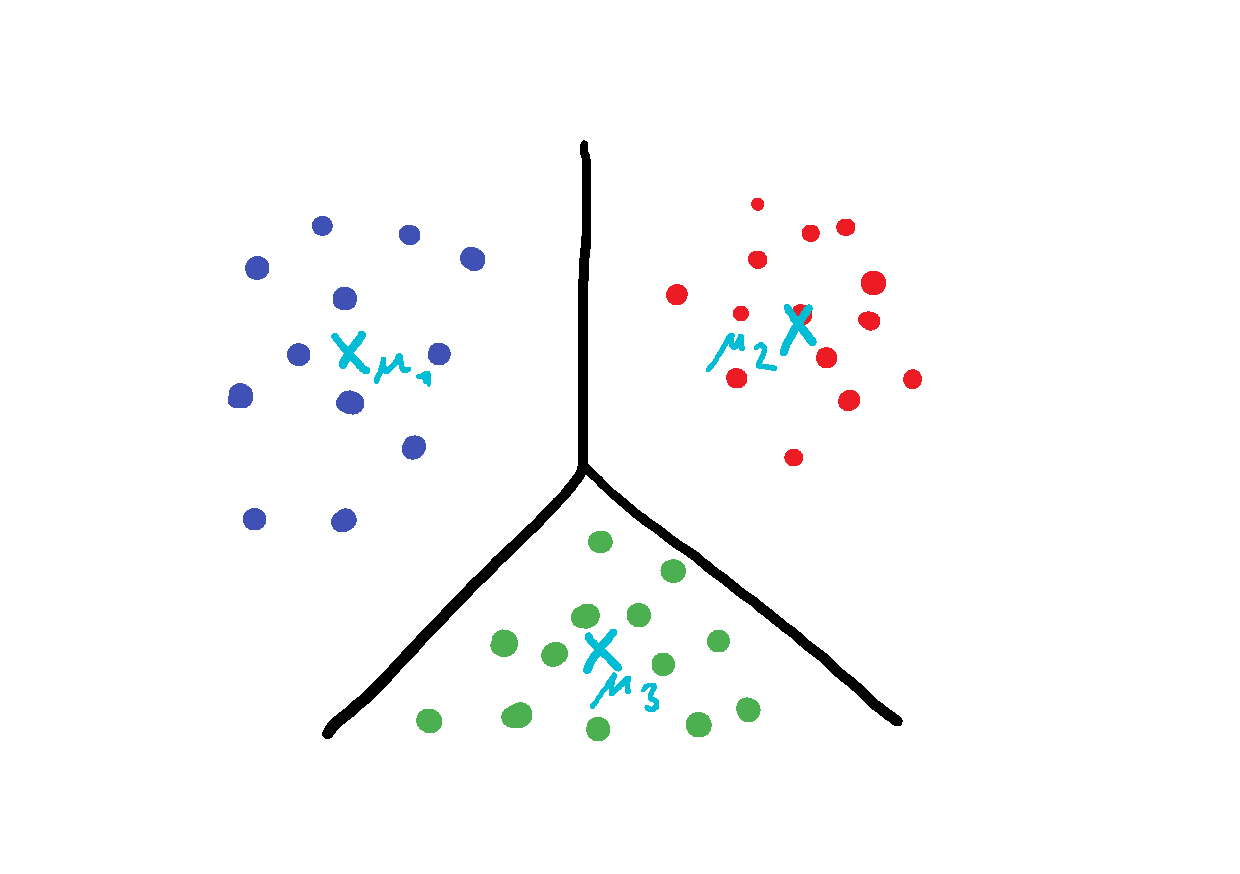
\includegraphics[height=5cm]{images/skizze_kmeans}
  \end{wrapfigure}
  \leavevmode
  \vspace{-1.0cm}
  \begin{itemize}
    \item Datenpunkte $\symbf{x_j}$ werden in $k$ \\ disjunkte Teilmengen $S_i$ partitioniert.
    \item Summierter quadratischer Fehler zu \\ Clusterzentren $\symbf{\mu_i}$ wird minnimiert
          \begin{equation*}
            \sum_{i=1}^{k} \sum_{\symbf{x_j} \in S_i} \lVert \symbf{x_j} - \symbf{\mu_i} \rVert^2 \rightarrow min.
          \end{equation*}
    \item Clusterzentren werden zunächst (zufällig) gewählt und dann iterativ aktualisiert.
  \end{itemize}
\end{frame}
% --- kmeans Clustering 1

% === Vorgehen
% --- Grundlagen 2
\begin{frame}{Vorgehen}
  \vspace{-0.8cm}
  \begin{center}
    \resizebox{13cm}{!}{%
      \includegraphics{images/transformationsbasierte_kompression/algorithm.tikz}
    }
  \end{center}
\end{frame}
% --- Grundlagen 2

% \begin{frame}{Vorgehen}
%   \begin{itemize}
%     \item Filter einer Faltungsschicht werden in Vektoren transformiert:
%     \begin{itemize}
%       \item jeder Filter separat (z.B. bei $3 \times 3$ Filtern)
%       \item mehrere Filter werden konkateniert (z.B. bei $1 \times 1$ Filtern)
%     \end{itemize}
%     \item Die Vektoren werden mit der DCT/DWT transformiert.
%     \item Man erhält Koeffizienten verschiedener Subbänder:
%     \begin{itemize}
%       \item bei der DWT auf natürliche Art
%       \item bei der DCT werden die Koeffizienten künstlich gruppiert
%     \end{itemize}
%   \item In jedem Subband $S_i$ wird separat ein $k$-Means Clustering durchgeführt mit Paramter $k_i$.
%   \item Als Parameter erhält man die Koeffizienten der Clusterzentren und Indizes.
%   \end{itemize}
% \end{frame}

% === Experiment
\section{Evaluation}

\begin{frame}{Übersicht}
  \tableofcontents[currentsection]
\end{frame}

\begin{frame}{Datensätze}
  Es wurden zwei Datensätze in der Bildklassifikation verwendet:
  \begin{itemize}
    \item Fashion-MNIST
    \begin{itemize}
      \item Enthält $70000$ Graustufenbilder der Größe $28 \times 28$.
      \item Enthält $10$ Klassen verschiedener Kleidungsstücke.
      \item Wurde vom Versandhändler Zalando erstellt.
      \item Kann als Ersatz für MNIST genutzt werden.
    \end{itemize}
  \end{itemize}
  \begin{figure}
    \begin{subfigure}{1.4cm}
        \centering
        
\includegraphics{images/datasets/fashionmnist/fashion_mnist_0_0.png}
    \end{subfigure}
    \begin{subfigure}{1.4cm}
        \centering
        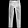
\includegraphics{images/datasets/fashionmnist/fashion_mnist_1_0.png}
    \end{subfigure}
    \begin{subfigure}{1.4cm}
        \centering
        
\includegraphics{images/datasets/fashionmnist/fashion_mnist_2_0.png}
    \end{subfigure}
    \begin{subfigure}{1.4cm}
        \centering
        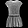
\includegraphics{images/datasets/fashionmnist/fashion_mnist_3_0.png}
    \end{subfigure}
    \begin{subfigure}{1.4cm}
        \centering
        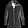
\includegraphics{images/datasets/fashionmnist/fashion_mnist_4_0.png}
    \end{subfigure}
    \par\bigskip
    \begin{subfigure}{1.4cm}
        \centering
        
\includegraphics{images/datasets/fashionmnist/fashion_mnist_5_0.png}
    \end{subfigure}
    \begin{subfigure}{1.4cm}
        \centering
        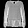
\includegraphics{images/datasets/fashionmnist/fashion_mnist_6_0.png}
    \end{subfigure}
    \begin{subfigure}{1.4cm}
        \centering
        
\includegraphics{images/datasets/fashionmnist/fashion_mnist_7_0.png}
    \end{subfigure}
    \begin{subfigure}{1.4cm}
        \centering
        
\includegraphics{images/datasets/fashionmnist/fashion_mnist_8_0.png}
    \end{subfigure}
    \begin{subfigure}{1.4cm}
        \centering
        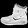
\includegraphics{images/datasets/fashionmnist/fashion_mnist_9_0.png}
    \end{subfigure}
  \end{figure}
\end{frame}

\begin{frame}
  \begin{itemize}
    \item CIFAR-10
    \begin{itemize}
      \item Enthält $60000$ Farbbilder der Größe $32 \times 32$.
      \item Enthält $10$ Klassen verschiedener Tiere und Verkehrsmittel.
      \item Ist Teilmenge des CIFAR-100 Datensatzes.
      \item Wurde aus dem 80 Million Tiny Images Datensatz generiert.
    \end{itemize}
  \end{itemize}
  \begin{figure}
    \begin{subfigure}{1.4cm}
        \centering
        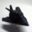
\includegraphics{images/datasets/cifar10/cifar_10_0_0.png}
    \end{subfigure}
    \begin{subfigure}{1.4cm}
        \centering
        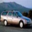
\includegraphics{images/datasets/cifar10/cifar_10_1_0.png}
    \end{subfigure}
    \begin{subfigure}{1.4cm}
        \centering
        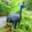
\includegraphics{images/datasets/cifar10/cifar_10_2_0.png}
    \end{subfigure}
    \begin{subfigure}{1.4cm}
        \centering
        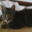
\includegraphics{images/datasets/cifar10/cifar_10_3_0.png}
    \end{subfigure}
    \begin{subfigure}{1.4cm}
        \centering
        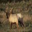
\includegraphics{images/datasets/cifar10/cifar_10_4_0.png}
    \end{subfigure}
    \par\bigskip
    \begin{subfigure}{1.4cm}
        \centering
        
\includegraphics{images/datasets/cifar10/cifar_10_5_0.png}
    \end{subfigure}
    \begin{subfigure}{1.4cm}
        \centering
        
\includegraphics{images/datasets/cifar10/cifar_10_6_0.png}
    \end{subfigure}
    \begin{subfigure}{1.4cm}
        \centering
        
\includegraphics{images/datasets/cifar10/cifar_10_7_0.png}
    \end{subfigure}
    \begin{subfigure}{1.4cm}
        \centering
        
\includegraphics{images/datasets/cifar10/cifar_10_8_0.png}
    \end{subfigure}
    \begin{subfigure}{1.4cm}
        \centering
        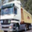
\includegraphics{images/datasets/cifar10/cifar_10_9_0.png}
    \end{subfigure}
  \end{figure}
\end{frame}

\begin{frame}{Netzarchitekturen}
  Es wurden zwei Netzarchitekturen untersucht:
  \begin{itemize}
    \item ResNet-20
    \begin{itemize}
      \item Erhöhung der Tiefe von Netzen führt zu Problemen.
      \item Residuenblöcke werden genutzt.
      \item Hat $271098$ Parameter für CIFAR-10 ($98{,}8\%$ in Faltungsschichten).
      \item Enthält nur $3 \times 3$ Faltungen.
    \end{itemize}
    \item MobileNet v2
    \begin{itemize}
      \item Enthält Residuenblöcke mit \glqq Depthwise Convolutions\grqq{}.
      \item Es folgen $1 \times 1$ Faltungsschichten.
      \item Enthält $1{,}3$ Mio. Parameter für CIFAR-10 ($95{,}3\%$ in Faltungsschichten).
    \end{itemize}
  \end{itemize}
\end{frame}

\begin{frame}{Ausführung auf Mikrocontrollern}
  Zur Ausführung von TensorFlow Modellen auf Mikrocontrollern stehen unter anderem zwei Alternativen zur Verfügung:
  \begin{itemize}
    \item TFLM
    \begin{itemize}
      \item TensorFlow Modell wird zunächst in ein TensorFlow Lite Modell konvertiert.
      \item Aus Clusterzentren und Indizes werden Gewichte der Originalgröße rekonstruiert.
      % \item Die Kompression geht dabei verloren.
      \item Im Rahmen der Arbeit daher nicht verwendbar.
    \end{itemize}
    \item IREE
    \begin{itemize}
      \item Verwendet Compiler Infrastruktur MLIR.
      \item Transformiert TensorFlow durch viele Konvertierungen in LLVM Code.
      \item IREE Bare-Metal-Arm zur Ausführung auf Mikrocontrollern mit Arm Prozessoren.
    \end{itemize}
  \end{itemize}
\end{frame}

\begin{frame}{Rekonstruktionsfehler}
  % Zunächst wird der reine Rekonstruktionsfehler der Gewichte untersucht:
  \begin{itemize}
    \item Parameter $k_i$ für $k$-Means Clustering werden durch relative Größen $c_i$ ersetzt.
    \item Transformation in zwei Subbänder (Approximations- und Detailkoeffizienten).
    \item Originalgewichte $W$ werden mit Parametern $(c_0, c_1)$ komprimiert.
    \item Gewichte $\widetilde{W}$ werden rekonstruiert.
    \item Normierter quadratischer Rekonstruktionsfehler gegeben durch
  \end{itemize}
  \begin{small}
    \begin{equation*}
      \NSE(W, \widetilde{W}) = \frac{\left\lVert \widetilde{W} - W \right\rVert_2^2}{\left\lVert W \right\rVert_2^2}.
    \end{equation*}
  \end{small}
  \begin{itemize}
    \item Kompressionsfaktor $r$ ist Quotient aus dem Speicherbedarf der Originalparameter und dem der komprimierten Parameter.
  \end{itemize}
  
\end{frame}

\begin{frame}{ResNet-20 für CIFAR-10}
  \begin{itemize}
    \item Die erste Faltungsschicht des 5. Residuenblocks wird komprimiert.
    \item Die Schicht hat $32$ Eingabe- und $32$ Ausgabekanäle.
    \item Dies entspricht $1024$ Filtern der Größe $3 \times 3$.
    \item Parameter $c_0$ und $c_1$ werden jeweils aus $\left\lbrace 0{,}1; 0{,}2; 0{,}4; 0{,}8 \right\rbrace$ gewählt.
    \item Größe der Subbänder ist
  \end{itemize}
  \begin{table}[H]
    \centering
    \begin{tabular}{|c|c|c|c|c|c|}
        \hline
        \multicolumn{2}{|c|}{DCT} & \multicolumn{2}{|c|}{DWT[HAAR]} & \multicolumn{2}{|c|}{DWT[DB2]} \\
        \hline
        $\left\lvert a \right\rvert$ & $\left\lvert d \right\rvert$ & $\left\lvert a \right\rvert$ & $\left\lvert d \right\rvert$ & $\left\lvert a \right\rvert$ & $\left\lvert d \right\rvert$ \\
        \hline
        5 & 4 & 5 & 5 & 6 & 6 \\
        \hline
    \end{tabular}
\end{table}
\end{frame}

\begin{frame}{Rekonstruktionsfehler ResNet-20 für Fashion-MNIST}
  \begin{figure}
    \resizebox{12.5cm}{!}{%
        \begin{subfigure}{0.5\textwidth}
            \centering
            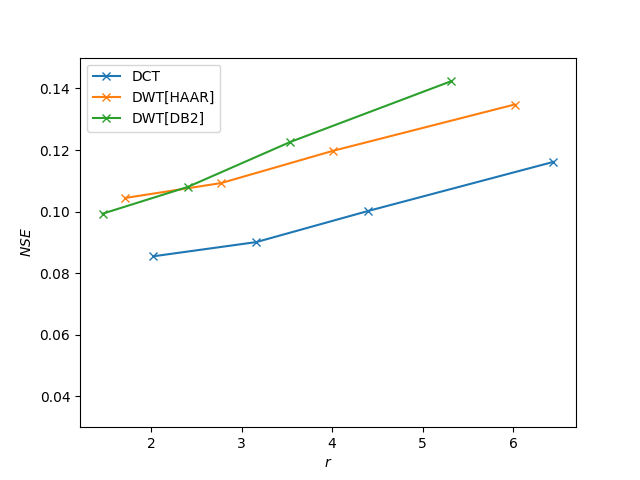
\includegraphics[width=\textwidth]{images/evaluation/reconstruction_error/cifar_10_resnet_20_47_nse_fixed_c1_0.1.tikz}
            \caption*{$c_1 = 0{,}1$ fest, $c_0$ variabel}
        \end{subfigure}
        \qquad
        \begin{subfigure}{0.5\textwidth}
            \centering
            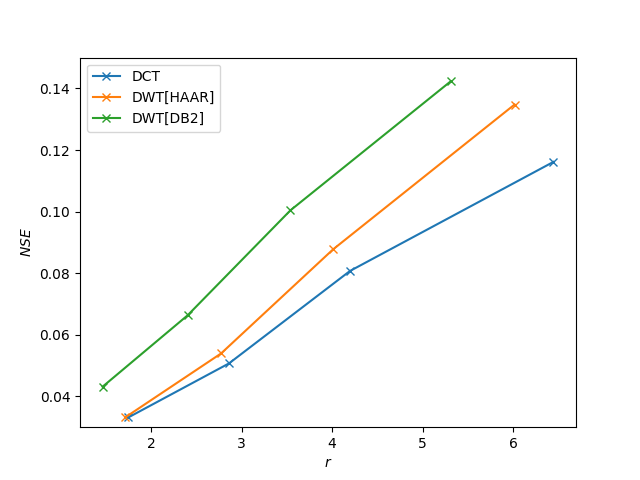
\includegraphics[width=\textwidth]{images/evaluation/reconstruction_error/cifar_10_resnet_20_47_nse_fixed_c0_0.1.tikz}
            \caption*{$c_0 = 0{,}1$ fest, $c_1$ variabel}
        \end{subfigure}
    }
    % \caption*{Normierter quadratischer Rekonstruktionsfehler der Gewichte einer Faltungsschicht eines \emph{ResNet-20} für den \emph{CIFAR-10} Datensatz für festes $c_1$ (a) bzw. festes $c_0$ (b) mit einem Wert von $0{,}1$.} 
\end{figure}
\end{frame}

\begin{frame}{Rekonstruktionsfehler ResNet-20 für Fashion-MNIST}
  \begin{wrapfigure}{r}{7cm}
    \vspace{-1.7cm}
    % \resizebox{7cm}{!}{
      \begin{figure}
        \resizebox{6cm}{!}{
          \begin{subfigure}{0.5\textwidth}
            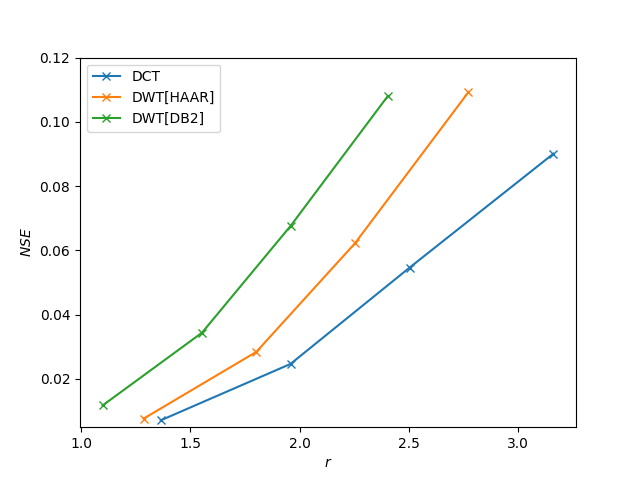
\includegraphics{images/evaluation/reconstruction_error/cifar_10_resnet_20_47_nse_fixed_c0_0.4.tikz}
            \subcaption*{$c_0 = 0{,}4$ fest, $c_1$ variabel}
          \end{subfigure}
        }
        % \caption*{$c_0 = 0{,}4$ fest, $c_1$ variabel}
      \end{figure}
    % }
    % 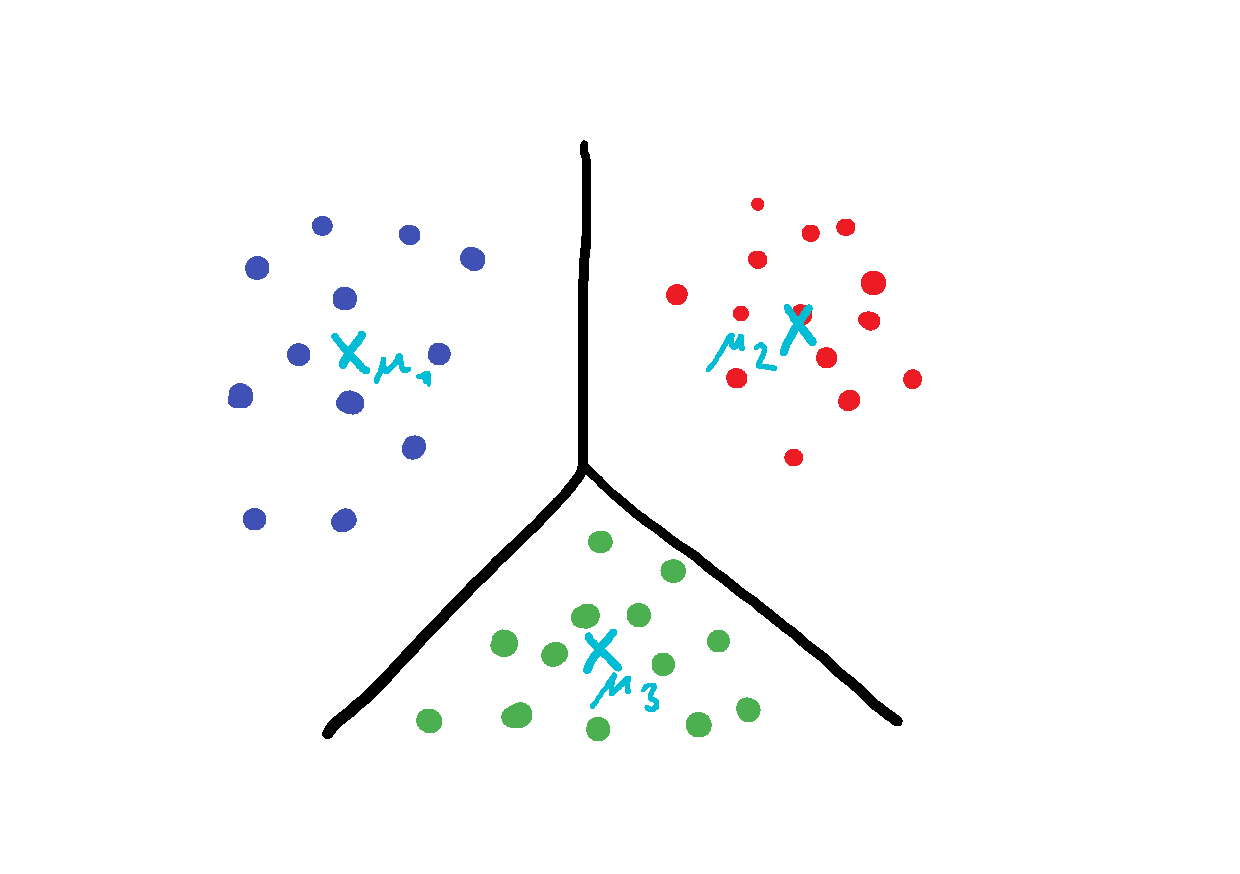
\includegraphics[height=5cm]{images/skizze_kmeans}
  \end{wrapfigure}
  \leavevmode
  \vspace{-1.0cm}
  \begin{itemize}
    \item Rekonstruktionsfehler ist für DCT am geringsten und für DB2 Wavelets am höchsten.
    \item Approximationskoeffizienten haben größeren Einfluss auf den Fehler als Detailkoeffizienten.
    \item Detailkoeffizienten können nicht gänzlich vernachlässigt werden.
  \end{itemize}
\end{frame}

\begin{frame}{Klassifikationsgenauigkeit ResNet-20 für Fashion-MNIST}
  % Zunächst wird der reine Rekonstruktionsfehler der Gewichte untersucht:
  \begin{itemize}
    \item Parameter und Kompressionsfaktor werden wie zuvor definiert.
    \item Alle Schichten werden mit dem selben Parameterpaar $(c_0, c_1)$ komprimiert.
    \item Das Netz wird für $20$ Epochen nachtrainiert.
    \item Parameter $c_0$ und $c_1$ werden jeweils aus $\left\lbrace 0{,}025; 0{,}05; 0{,}1; 0{,}2; 0{,}4; 0{,}8; 1{,}0 \right\rbrace$ gewählt.
    \item Genauigkeit des Originalnetzes liegt bei $94{,}7\%$.
    % \item Es werden hohhe Kompressionsraten ohne nennenswerten Genauigkeitsverlust erreicht.
    % \item Auch hier sind Approximationskoeffizienten von größerer Wichtigkeit.
  \end{itemize}  
\end{frame}

\begin{frame}{Klassifikationsgenauigkeit ResNet-20 für Fashion-MNIST}
  \begin{figure}
    \resizebox{12cm}{!}{%
        \begin{subfigure}{0.5\textwidth}
            \centering
            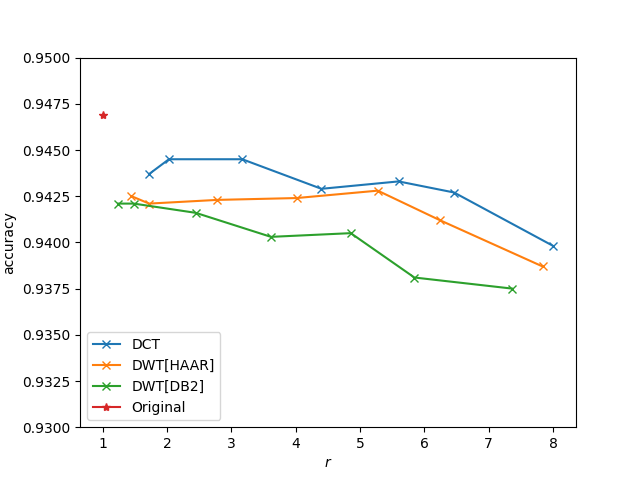
\includegraphics[width=\textwidth]{images/evaluation/accuracy/fashion_mnist_resnet_20_fine_tuned_accuracy_fixed_c1_0.05.tikz}
            \caption*{$c_1 = 0{,}05$ fest, $c_0$ variabel}
        \end{subfigure}
        \qquad
        \begin{subfigure}{0.5\textwidth}
            \centering
            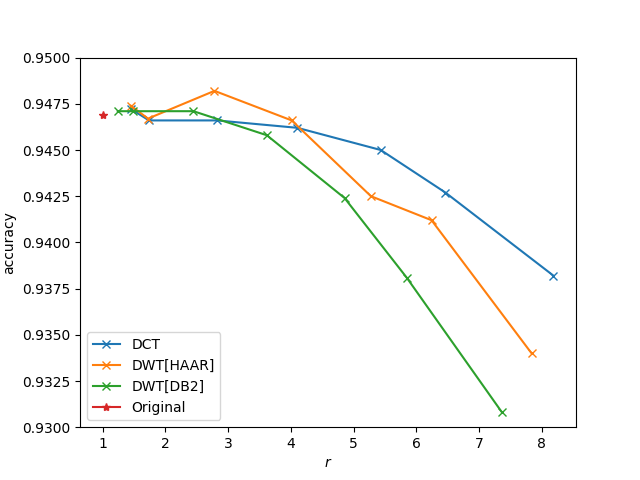
\includegraphics[width=\textwidth]{images/evaluation/accuracy/fashion_mnist_resnet_20_fine_tuned_accuracy_fixed_c0_0.05.tikz}
            \caption*{$c_0 = 0{,}05$ fest, $c_1$ variabel}
        \end{subfigure}
    }
    % \caption*{Normierter quadratischer Rekonstruktionsfehler der Gewichte einer Faltungsschicht eines \emph{ResNet-20} für den \emph{CIFAR-10} Datensatz für festes $c_1$ (a) bzw. festes $c_0$ (b) mit einem Wert von $0{,}1$.} 
\end{figure}
\end{frame}

\begin{frame}{Klassifikationsgenauigkeit MobileNet v2 für CIFAR-10}
  % Zunächst wird der reine Rekonstruktionsfehler der Gewichte untersucht:
  \begin{itemize}
    \item Genauigkeit des Originalnetzes liegt bei $89{,}4\%$.
    \item Parameter $c_0$ und $c_1$ werden jeweils aus $\left\lbrace 0{,}025; 0{,}05; 0{,}1; 0{,}2 \right\rbrace$ gewählt.
    \item Speicherbedarf während des Trainigs sehr hoch:
    \begin{itemize}
      \item 32${\,}$GB einer Tesla Grafikkarte reichen nicht aus für größere Werte von $c_0$ und $c_1$
    \end{itemize}
  \item Parameterraum wird nur teilweise abgedeckt.
  % \item Genauigkeit des Originalnetzes kann nicht erreicht werden:
  % \begin{itemize}
  %   \item Kompressionsfaktor von etwa 3 jedoch Genauigkeitsverlust von 5 Prozentpunkten
  % \end{itemize}
  \end{itemize}  
\end{frame}

\begin{frame}{Klassifikationsgenauigkeit MobileNet v2 für CIFAR-10}
  \begin{figure}
    \resizebox{12cm}{!}{%
        \begin{subfigure}{0.5\textwidth}
            \centering
            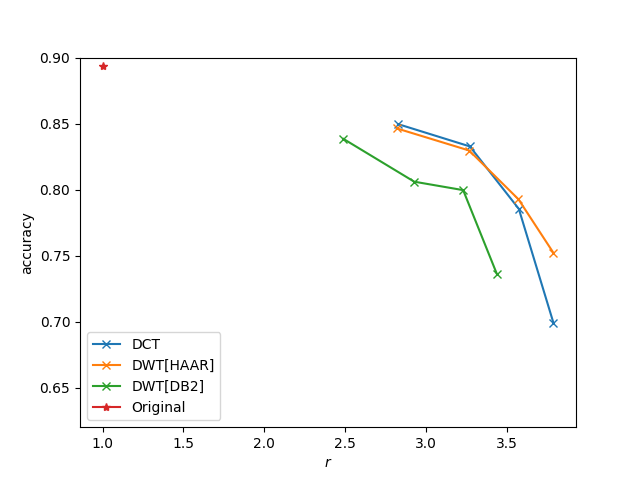
\includegraphics[width=\textwidth]{images/evaluation/accuracy/cifar_10_mobilenet_v2_filterwise_or_vector8_fine_tuned_accuracy_fixed_c1_0.2.tikz}
            \caption*{$c_1 = 0{,}2$ fest, $c_0$ variabel}
        \end{subfigure}
        \qquad
        \begin{subfigure}{0.5\textwidth}
            \centering
            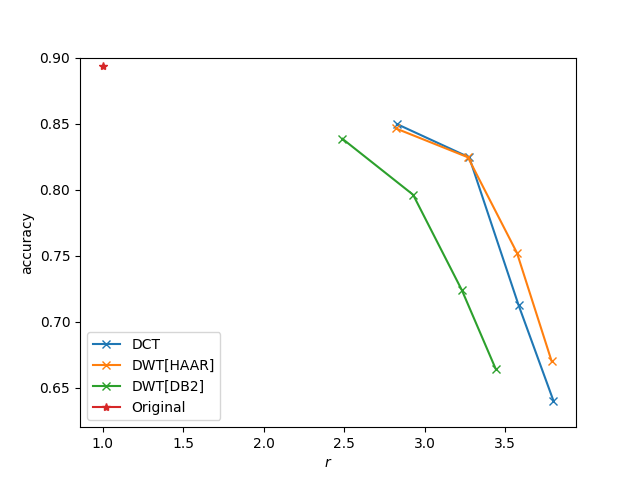
\includegraphics[width=\textwidth]{images/evaluation/accuracy/cifar_10_mobilenet_v2_filterwise_or_vector8_fine_tuned_accuracy_fixed_c0_0.2.tikz}
            \caption*{$c_0 = 0{,}2$ fest, $c_1$ variabel}
        \end{subfigure}
    }
    % \caption*{Normierter quadratischer Rekonstruktionsfehler der Gewichte einer Faltungsschicht eines \emph{ResNet-20} für den \emph{CIFAR-10} Datensatz für festes $c_1$ (a) bzw. festes $c_0$ (b) mit einem Wert von $0{,}1$.} 
\end{figure}
\end{frame}

\begin{frame}{Klassifikationsgenauigkeit MobileNet v2 für CIFAR-10}
  \begin{wrapfigure}{r}{7cm}
    \vspace{-1.7cm}
    % \resizebox{7cm}{!}{
      \begin{figure}
        \resizebox{6cm}{!}{
          \begin{subfigure}{0.5\textwidth}
            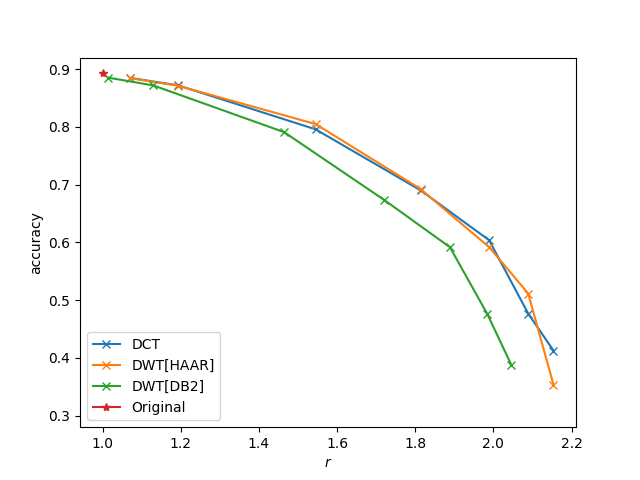
\includegraphics{images/evaluation/accuracy/cifar_10_mobilenet_v2_filterwise4_or_vector32_fine_tuned_accuracy_fixed_c0_0.8.tikz}
            \subcaption*{$c_0 = 0{,}8$ fest, $c_1$ variabel}
          \end{subfigure}
        }
        % \caption*{$c_0 = 0{,}4$ fest, $c_1$ variabel}
      \end{figure}
    % }
    % 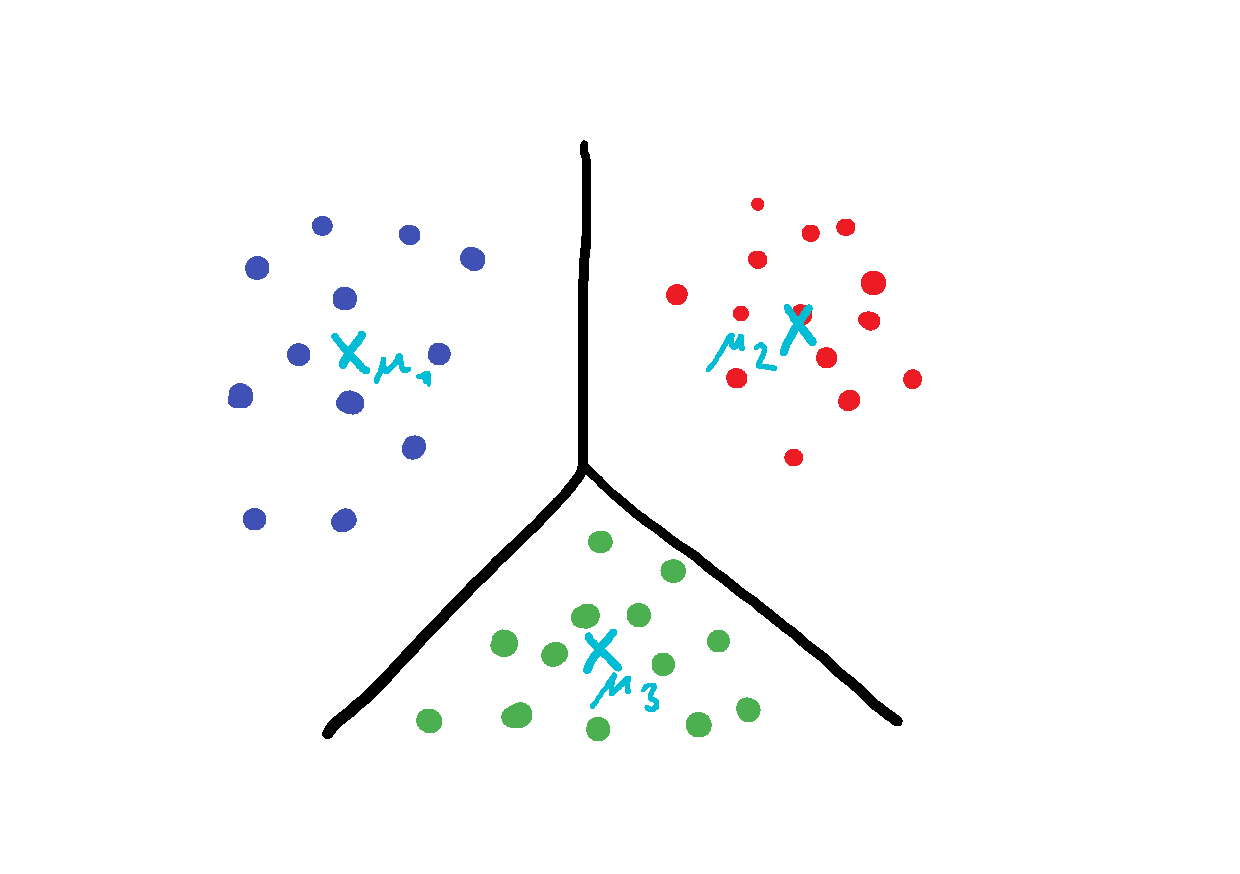
\includegraphics[height=5cm]{images/skizze_kmeans}
  \end{wrapfigure}
  \leavevmode
  \vspace{-1.0cm}
  \begin{itemize}
    \item Ressourcenbedarf für das \\ Training kann durch Konkatenation von mehr Filtern gesenkt werden.
    \item Parameterraum kann \\ im Gesamten abgesucht werden.
    \item Es wird keine nennenswerte \\ Kompression erreicht.
    \item Gittersuche ist bei diesem \\ Netz so nicht zielführend.
  \end{itemize}
\end{frame}

\begin{frame}{Komprimierbarkeit einzelner Schichten}
  % Zunächst wird der reine Rekonstruktionsfehler der Gewichte untersucht:
  \begin{itemize}
    \item Es ist nicht zu erwawrten, dass sich alle Faltungsschichten gleich gut komprimieren lassen.
    \item Gittersuche ist sehr rechenaufwendig.
    \item Wie lassen sich gezielter geeignete Parameter einzelner Schichten identifizieren?
    \begin{itemize}
      \item Komprimiere jeweils nur eine Schicht bei der Gittersuche.
      \item \glqq Freeze\grqq{} die übrigen Schichten.
      \item Dies ist deutlich ressourcenschonender und schneller.
      \item Wähle die kleinsten Kompressionsparameter, sodass eine Schranke für den Genauigkeitsverlust $\Delta \acc$ nicht überschritten wird.
    \end{itemize}
  \end{itemize}  
\end{frame}

\begin{frame}{Absolute Speichergröße MobileNet v2 für CIFAR-10}
  \vspace{0.2cm}
  \begin{figure}
    \resizebox{13cm}{!}{%
      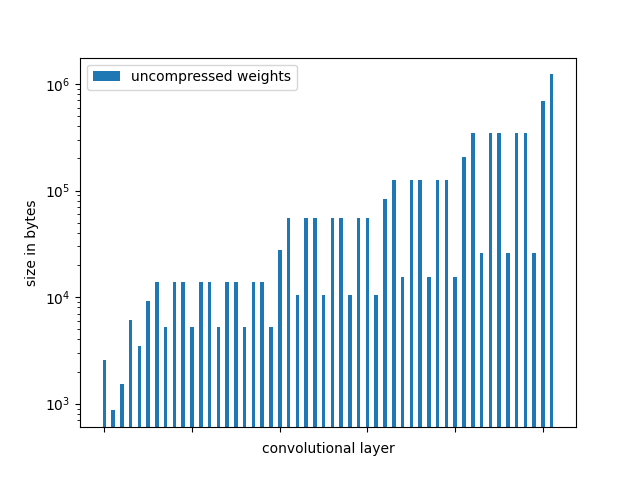
\includegraphics{images/evaluation/layerwise/cifar_10_mobilenet_v2_absolute_uncompressed.tikz}
    }
    \caption*{Absolute Speichergröße der Faltungsschichten.}
  \end{figure}
\end{frame}

\begin{frame}{Relative Speichergröße MobileNet v2 für CIFAR-10}
  \vspace{0.2cm}
  \begin{figure}
    \resizebox{13cm}{!}{%
      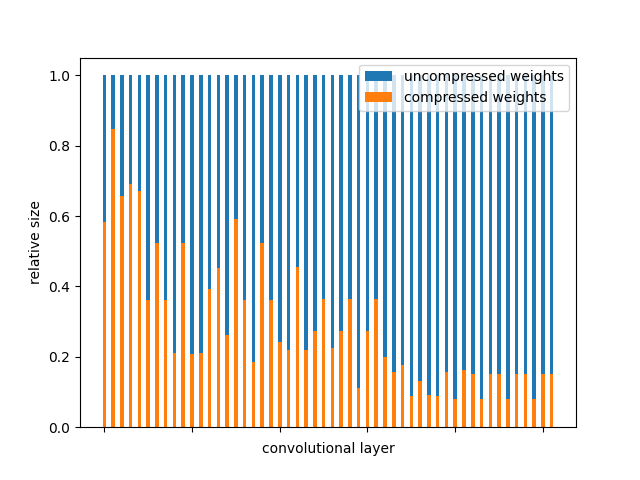
\includegraphics{images/evaluation/layerwise/cifar_10_mobilenet_v2_DCT_relative_0.0025.tikz}
    }
    \caption*{Relative Speichergröße der Faltungsschichten für $\Delta \acc = 0{,}0025$.}
  \end{figure}
\end{frame}

\begin{frame}{Adaptive Kompression MobileNet v2 für CIFAR-10}
  \begin{table}[H]
    \centering
    % \caption{Genauigkeiten und Kompressionsfaktoren für ein \emph{MobileNet v2} für den \emph{CIFAR-10} Datensatz für verschiedene maximale Genauigkeitsverluste $\Delta\acc$ und Transformationen.}
    % \label{table_evaluation_layerwise_cifar10_mobilenet}
    \begin{tabular}{|l|ll|ll|}
    \hline
           & \multicolumn{2}{l|}{\textbf{DCT}}             & \multicolumn{2}{l|}{\textbf{DWT{[}HAAR{]}}}   \\ \hline
    $\Delta\text{acc}$    & \multicolumn{1}{l|}{$\acc$} & $r$  & \multicolumn{1}{l|}{$\acc$} & $r$  \\ \hline
    $0{,}0025$ & \multicolumn{1}{l|}{$86{,}15\%$}  & $4{,}93$ & \multicolumn{1}{l|}{$86{,}31\%$}  & $4{,}97$  \\ \hline
    $0{,}005$  & \multicolumn{1}{l|}{$84{,}31\%$}  & $5{,}34$ & \multicolumn{1}{l|}{$84{,}5\%$}   & $5{,}33$ \\ \hline
    \end{tabular}
\end{table}
\pause
\begin{itemize}
  \item Klassifikationsgenauigkeit ist höher als bei der Gittersuche.
  \item Es wird Kompressiosnfaktor 5 statt 3 erreicht.
  \item Verfahren erlaubt feinere Parametersuche.
\end{itemize}
\end{frame}

\begin{frame}{Firmwaregröße}
  \begin{itemize}
    \item Für die Ausführung auf Mikrocontrollern darf die Firmwaregröße den Flash Speicher des Controllers nicht übersteigen.
    \item Dieser liegt bei STM32 Nucleo Boards im Bereich bis etwa 2$\,$MB.
    \item Setzt sich zusammen aus:
    \begin{itemize}
      \item Initialisierung des Mikrocontrollers
      \item IREE Runtime
      \item Gewichte und Code zur Ausführung (Netzschichten, inverse DCT/DWT)
    \end{itemize}
  \end{itemize}
\end{frame}

\begin{frame}{Firmwaregröße ResNet-20 für Fashion-MNIST}
  \begin{figure}
    \resizebox{12cm}{!}{%
        \begin{subfigure}{0.5\textwidth}
            \centering
            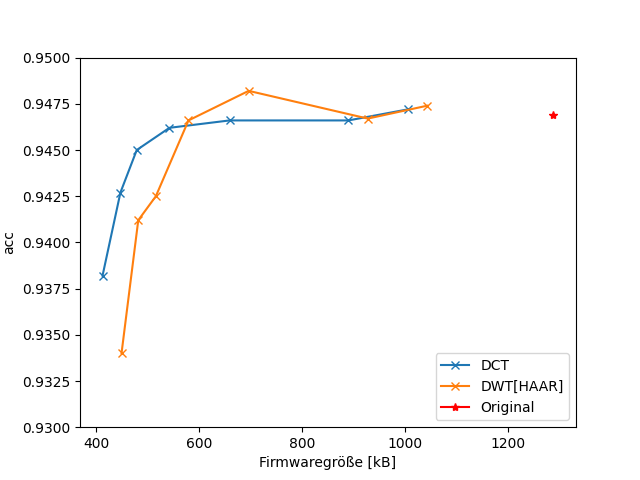
\includegraphics[width=\textwidth]{images/evaluation/binary_size/fashion_mnist_resnet_20_filterwise_or_vector8_acc_vs_filesize_fixed_c0_0.05.tikz}
            \caption*{$c_0 = 0{,}2$ fest, $c_1$ variabel}
        \end{subfigure}
        \qquad
        \begin{subfigure}{0.5\textwidth}
            \centering
            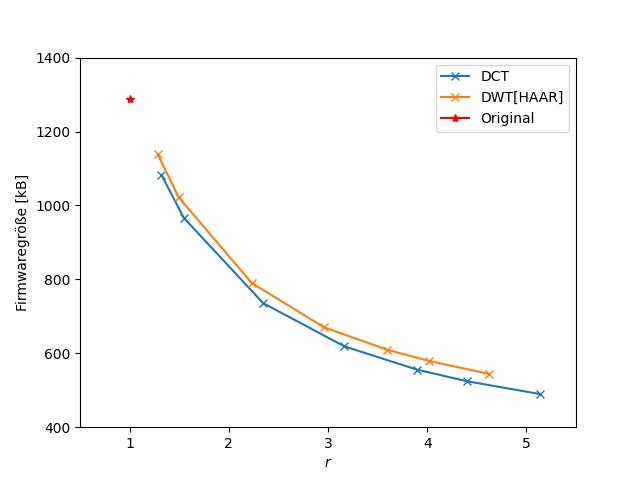
\includegraphics[width=\textwidth]{images/evaluation/binary_size/fashion_mnist_resnet_20_filterwise_or_vector8_filesize_vs_compression_fixed_c0_0.2.tikz}
            \caption*{$c_0 = 0{,}2$ fest, $c_1$ variabel}
        \end{subfigure}
    }
    % \caption*{Normierter quadratischer Rekonstruktionsfehler der Gewichte einer Faltungsschicht eines \emph{ResNet-20} für den \emph{CIFAR-10} Datensatz für festes $c_1$ (a) bzw. festes $c_0$ (b) mit einem Wert von $0{,}1$.} 
\end{figure}
\end{frame}

\begin{frame}{Firmwaregröße MobileNet v2 für CIFAR-10}
  \begin{table}[H]
    \centering
    % \caption{Genauigkeiten und Firmwaregrößen (FW-Größe) in Kilobytes für verschieden komprimierte \emph{MobileNet v2} für den \emph{CIFAR-10} Datensatz. Verglichen werden das unkomprimierte Netz (a), ein in allen Faltungsschichten gleich komprimiertes Netz (b) und ein adaptiv komprimiertes Netz (c) (vgl. Abschnitt \ref{layer_compressing}).}
    % \label{table_evaluation_file_size_cifar_10_mobilenet}
    \begin{tabular}{|c|cc|cc|}
        \hline
                                        & \multicolumn{2}{c|}{\textbf{DCT}}                                            & \multicolumn{2}{c|}{\textbf{DWT{[}HAAR{]}}}                                  \\ \hline
        \textbf{Konfiguration}          & \multicolumn{1}{c|}{\textbf{$\text{acc}$}} & \textbf{FW-Größe {[}kB{]}} & \multicolumn{1}{c|}{\textbf{$\text{acc}$}} & \textbf{FW-Größe {[}kB{]}} \\ \hline
        unkomprimiert               & \multicolumn{1}{c|}{$89{,}36\%$}           & $5701{,}71$                     & \multicolumn{1}{c|}{$89{,}36\%$}           & $5701{,}71$                     \\ \hline
        $c_0=0{,}2, c_1=0{,}2$      & \multicolumn{1}{c|}{$84{,}96\%$}           & $2325{,}14$                     & \multicolumn{1}{c|}{$84{,}63\%$}           & $2425{,}57$                     \\ \hline
        $\Delta\text{acc}=0{,}0025$ & \multicolumn{1}{c|}{$86{,}15\%$}           & $1510{,}78$                     & \multicolumn{1}{c|}{$86{,}31\%$}           & $1601{,}89$                     \\ \hline
        \end{tabular}
\end{table}
\pause
\begin{itemize}
  \item Deutliche Reduzierung der Firmwaregröße wird erzielt.
  \item Verläuft u.A. wegen IREE Runtime nicht linear zum Kompressionsfaktor.
  % \item 
\end{itemize}
\end{frame}

\begin{frame}{Arbeitsspeicherbedarf}
  \begin{itemize}
    \item Auch der verfügbare Arbeitsspeicher ist ein limitierender Faktor.
    \item Die Gewichte einer Faltungsschicht werden vollständig rekonstruiert.
    \item Es hat sich gezeigt, dass der Arbeitsspeicherbedarf deutlich ansteigt.
    \item Probleme liegen teilweise in der Verwendung von IREE.
    \item Die Netze wurden mit dem Emulator Renode ausgeführt.
  \end{itemize}
\end{frame}

\begin{frame}{Arbeitsspeicherverbrauch MobileNet v2 für CIFAR-10}
  \begin{table}[H]
    \centering
    % \caption{Maximaler Arbeitsspeicherverbrauch in Kilobytes für verschieden komprimierte \emph{MobileNet v2} für den \emph{CIFAR-10} Datensatz. Verglichen werden das unkomprimierte Netz (a), in allen Faltungsschichten gleich komprimierte Netze (b) und ein adaptiv komprimiertes Netz (c) (vgl. Abschnitt \ref{layer_compressing}).}
    % \label{table_evaluation_peak_memory_cifar_10_mobilenet}
    \begin{tabular}{|c|c|c|}
        \hline
        \textbf{Konfiguration}          & \textbf{DCT} & \textbf{DWT{[}HAAR{]}} \\ \hline
        unkomprimiert               & $2390{,}29$  & $2390{,}29$            \\ \hline
        gleich in allen Schichten   & $4915{,}91$  & $12587{,}29$           \\ \hline
        $\Delta\text{acc}=0{,}0025$ & $6205{,}16$  & $12388{,}60$           \\ \hline
        \end{tabular}
\end{table}  
\pause
\begin{itemize}
  \item Deutlich mehr Arbeitsspeicherbedarf bei Verwendung der DWT
  \item Es werden nicht alle TensorFlow Operationen unterstützt (z.B. transposed convolution, inplace updates).
  % \item Erweiterung von IREE wäre nötig (nicht trivial).
  \item Ersetzung dieser Konstrukte auf TensorFlow Ebene durch ineffiziente Implementierungen (stacking von Tensoren, $\ldots$).
\end{itemize}
\end{frame}


% --- Experiment 1
% \begin{frame}{Erstes Experiment}
%   Die Kompressionseigenschaften der DCT und DWT werden an einem einfachen Beispiel untersucht.
%   \begin{itemize}
%     \item Gewichte einer Faltungsschicht eines trainierten CNNs werden komprimiert.
%     \item Mehrere Filter werden als ein Vektor aufgefasst, um die Signallänge zu erhöhen.
%     \item Diese werden jeweils mittels DCT bzw. DWT transformiert.
%     \item Transformierte werden auf die ersten $n$ (DCT) bzw. betraglich größten $n$ (DWT) \\ Koeffizienten beschränkt.
%     \item Transformationen werden invertiert.
%           % \item Norm des Fehlers
%           % \item erwarten bei gelicher Parameterzahl geringeren Fehler bei DWT
%           % \item bei DWT eine geringe Auswahl von Konfigurationen (Wavelet/Tiefe)
%   \end{itemize}
% \end{frame}
% --- Experiment 1

% --- Experiment 2
% \begin{frame}
%   \begin{wrapfigure}{l}{8cm}
%     \vspace{-0.8cm}
%     \resizebox{7.8cm}{!}{%
%       % This file was created with tikzplotlib v0.10.1.
\begin{tikzpicture}

\definecolor{darkgray176}{RGB}{176,176,176}
\definecolor{lightgray204}{RGB}{204,204,204}
\definecolor{steelblue31119180}{RGB}{31,119,180}

\begin{axis}[
legend style={fill opacity=0.8, draw opacity=1, text opacity=1, draw=lightgray204},
tick align=outside,
tick pos=left,
x grid style={darkgray176},
xlabel={\(\displaystyle t\)},
xmin=-1.15, xmax=2.15,
xtick style={color=black},
y grid style={darkgray176},
ylabel={\(\displaystyle \psi(t)\)},
ymin=-1.1, ymax=1.1,
ytick style={color=black}
]
\addplot [semithick, steelblue31119180, forget plot]
table {%
-1 0
-0.987951807228916 0
-0.975903614457831 0
-0.963855421686747 0
-0.951807228915663 0
-0.939759036144578 0
-0.927710843373494 0
-0.91566265060241 0
-0.903614457831325 0
-0.891566265060241 0
-0.879518072289157 0
-0.867469879518072 0
-0.855421686746988 0
-0.843373493975904 0
-0.831325301204819 0
-0.819277108433735 0
-0.807228915662651 0
-0.795180722891566 0
-0.783132530120482 0
-0.771084337349398 0
-0.759036144578313 0
-0.746987951807229 0
-0.734939759036145 0
-0.72289156626506 0
-0.710843373493976 0
-0.698795180722892 0
-0.686746987951807 0
-0.674698795180723 0
-0.662650602409639 0
-0.650602409638554 0
-0.63855421686747 0
-0.626506024096386 0
-0.614457831325301 0
-0.602409638554217 0
-0.590361445783133 0
-0.578313253012048 0
-0.566265060240964 0
-0.55421686746988 0
-0.542168674698795 0
-0.530120481927711 0
-0.518072289156627 0
-0.506024096385542 0
-0.493975903614458 0
-0.481927710843373 0
-0.469879518072289 0
-0.457831325301205 0
-0.44578313253012 0
-0.433734939759036 0
-0.421686746987952 0
-0.409638554216867 0
-0.397590361445783 0
-0.385542168674699 0
-0.373493975903614 0
-0.36144578313253 0
-0.349397590361446 0
-0.337349397590361 0
-0.325301204819277 0
-0.313253012048193 0
-0.301204819277108 0
-0.289156626506024 0
-0.27710843373494 0
-0.265060240963855 0
-0.253012048192771 0
-0.240963855421687 0
-0.228915662650602 0
-0.216867469879518 0
-0.204819277108434 0
-0.192771084337349 0
-0.180722891566265 0
-0.168674698795181 0
-0.156626506024096 0
-0.144578313253012 0
-0.132530120481928 0
-0.120481927710843 0
-0.108433734939759 0
-0.0963855421686747 0
-0.0843373493975903 0
-0.0722891566265059 0
-0.0602409638554217 0
-0.0481927710843373 0
-0.036144578313253 0
-0.0240963855421686 0
-0.0120481927710843 0
0 1
0.0120481927710845 1
0.0240963855421688 1
0.036144578313253 1
0.0481927710843375 1
0.0602409638554218 1
0.072289156626506 1
0.0843373493975905 1
0.0963855421686748 1
0.108433734939759 1
0.120481927710844 1
0.132530120481928 1
0.144578313253012 1
0.156626506024097 1
0.168674698795181 1
0.180722891566265 1
0.192771084337349 1
0.204819277108434 1
0.216867469879518 1
0.228915662650602 1
0.240963855421687 1
0.253012048192771 1
0.265060240963855 1
0.27710843373494 1
0.289156626506024 1
0.301204819277108 1
0.313253012048193 1
0.325301204819277 1
0.337349397590361 1
0.349397590361446 1
0.36144578313253 1
0.373493975903614 1
0.385542168674699 1
0.397590361445783 1
0.409638554216867 1
0.421686746987952 1
0.433734939759036 1
0.44578313253012 1
0.457831325301205 1
0.469879518072289 1
0.481927710843373 1
0.493975903614458 1
0.506024096385542 -1
0.518072289156627 -1
0.530120481927711 -1
0.542168674698795 -1
0.55421686746988 -1
0.566265060240964 -1
0.578313253012048 -1
0.590361445783133 -1
0.602409638554217 -1
0.614457831325301 -1
0.626506024096386 -1
0.63855421686747 -1
0.650602409638554 -1
0.662650602409639 -1
0.674698795180723 -1
0.686746987951807 -1
0.698795180722892 -1
0.710843373493976 -1
0.72289156626506 -1
0.734939759036145 -1
0.746987951807229 -1
0.759036144578313 -1
0.771084337349398 -1
0.783132530120482 -1
0.795180722891566 -1
0.807228915662651 -1
0.819277108433735 -1
0.831325301204819 -1
0.843373493975904 -1
0.855421686746988 -1
0.867469879518072 -1
0.879518072289157 -1
0.891566265060241 -1
0.903614457831325 -1
0.91566265060241 -1
0.927710843373494 -1
0.939759036144578 -1
0.951807228915663 -1
0.963855421686747 -1
0.975903614457831 -1
0.987951807228916 -1
1 0
1.01204819277108 0
1.02409638554217 0
1.03614457831325 0
1.04819277108434 0
1.06024096385542 0
1.07228915662651 0
1.08433734939759 0
1.09638554216868 0
1.10843373493976 0
1.12048192771084 0
1.13253012048193 0
1.14457831325301 0
1.1566265060241 0
1.16867469879518 0
1.18072289156627 0
1.19277108433735 0
1.20481927710843 0
1.21686746987952 0
1.2289156626506 0
1.24096385542169 0
1.25301204819277 0
1.26506024096386 0
1.27710843373494 0
1.28915662650602 0
1.30120481927711 0
1.31325301204819 0
1.32530120481928 0
1.33734939759036 0
1.34939759036145 0
1.36144578313253 0
1.37349397590361 0
1.3855421686747 0
1.39759036144578 0
1.40963855421687 0
1.42168674698795 0
1.43373493975904 0
1.44578313253012 0
1.4578313253012 0
1.46987951807229 0
1.48192771084337 0
1.49397590361446 0
1.50602409638554 0
1.51807228915663 0
1.53012048192771 0
1.5421686746988 0
1.55421686746988 0
1.56626506024096 0
1.57831325301205 0
1.59036144578313 0
1.60240963855422 0
1.6144578313253 0
1.62650602409639 0
1.63855421686747 0
1.65060240963855 0
1.66265060240964 0
1.67469879518072 0
1.68674698795181 0
1.69879518072289 0
1.71084337349398 0
1.72289156626506 0
1.73493975903614 0
1.74698795180723 0
1.75903614457831 0
1.7710843373494 0
1.78313253012048 0
1.79518072289157 0
1.80722891566265 0
1.81927710843373 0
1.83132530120482 0
1.8433734939759 0
1.85542168674699 0
1.86746987951807 0
1.87951807228916 0
1.89156626506024 0
1.90361445783133 0
1.91566265060241 0
1.92771084337349 0
1.93975903614458 0
1.95180722891566 0
1.96385542168675 0
1.97590361445783 0
1.98795180722892 0
2 0
};
\end{axis}

\end{tikzpicture}

%     }
%   \end{wrapfigure}
%   \leavevmode
%   \begin{itemize}
%     \item Gewichte $W$ einer Faltungsschicht \\ aus einem ResNet18
%     \item 512 Filter der Größe $3 \times 3$
%     \item Gruppierung von jeweils \\ 4 Filtern zu 128 Vektoren der \\ Länge 36
%     \item Haar Wavelet für die DWT
%     \item Nur 2 Subbänder $a_0$ und $d_0$ (Level 1)
%   \end{itemize}
% \end{frame}
% --- Experiment 2

% --- Experiment 3
% \begin{frame}
%   \begin{wrapfigure}{l}{8cm}
%     \vspace{-0.8cm}
%     \resizebox{7.8cm}{!}{%
%       % This file was created with tikzplotlib v0.10.1.
\begin{tikzpicture}

\definecolor{darkgray176}{RGB}{176,176,176}
\definecolor{darkorange25512714}{RGB}{255,127,14}
\definecolor{lightgray204}{RGB}{204,204,204}
\definecolor{steelblue31119180}{RGB}{31,119,180}

\begin{axis}[
legend cell align={left},
legend style={
  fill opacity=0.8,
  draw opacity=1,
  text opacity=1,
  at={(0.97,0.03)},
  anchor=south east,
  draw=lightgray204
},
tick align=outside,
tick pos=left,
x grid style={darkgray176},
xlabel={Kompressionsfaktor},
xmin=0.6, xmax=9.4,
xtick style={color=black},
y grid style={darkgray176},
ylabel={Normalisierter Fehler 
 \(\displaystyle e_{rel}\)},
ymin=-0.046607475585386, ymax=0.978758379632833,
ytick style={color=black}
]
\addplot [semithick, steelblue31119180]
table {%
9 0.932150840759277
7.2 0.92421692609787
5.14285714285714 0.891453623771667
4 0.866038143634796
3.6 0.864060819149017
3 0.849342465400696
2.57142857142857 0.815710723400116
2.4 0.806412398815155
2.11764705882353 0.783090651035309
1.89473684210526 0.691582381725311
1.8 0.661345958709717
1.63636363636364 0.639122068881989
1.5 0.599117159843445
1.44 0.576391458511353
1.33333333333333 0.547637343406677
1.24137931034483 0.51213526725769
1.2 0.476507186889648
1.125 0.381945371627808
1.05882352941176 0.326091170310974
1 1.37568136437949e-07
};
\addlegendentry{DCT}
\addplot [semithick, darkorange25512714]
table {%
9 0.731678664684296
7.2 0.683795571327209
5.14285714285714 0.598288714885712
4 0.523815393447876
3.6 0.48941370844841
3 0.425979554653168
2.57142857142857 0.369816660881042
2.4 0.343426793813705
2.11764705882353 0.2943035364151
1.89473684210526 0.248749569058418
1.8 0.227121189236641
1.63636363636364 0.186587646603584
1.5 0.148958936333656
1.44 0.131311669945717
1.33333333333333 0.0975319966673851
1.24137931034483 0.0674435645341873
1.2 0.0545677915215492
1.125 0.0312185026705265
1.05882352941176 0.0139471152797341
1 6.32881693718446e-08
};
\addlegendentry{DWT [Haar; Level=1]}
\end{axis}

\end{tikzpicture}

%     }
%   \end{wrapfigure}
%   \leavevmode
%   \begin{itemize}
%     \item $dct(W; n)$ ist DCT Transformierte \\ mit ersten n Koeffizienten
%     \item $dwt(W; n)$ ist DWT Transformierte \\ mit betraglich n größten \\ Koeffizienten
%     \item $e_{\mathcal{T}}(n) = W - \mathcal{T}^{-1}(\mathcal{T}(W; n))$
%           % \item $e_{dwt}(n) = W - idwt(dwt(W; n))$
%     \item $e_{rel}(n) = \frac{\lVert e_{\mathcal{T}}(n) \rVert}{\lVert W \rVert}$
%   \end{itemize}
% \end{frame}
% --- Experiment 3
% === Experiment

% === Ausblick
\section{Zusammenfassung und Ausblick}

\begin{frame}{Übersicht}
  \tableofcontents[currentsection]
\end{frame}

% --- Ausblick 1
% \begin{frame}{Ausblick}
%   Neben den in der Motivation genannten Punkten sollen folgende Fragestellungen untersucht werden:
%   \begin{itemize}
%     \item Wie führt man das komprimierte Netz auf der Zielplattform aus?
%           \begin{itemize}
%             \item Die Rücktransformation aller Schichten zur selben Zeit ist nicht sinnvoll.
%             \item Gewichte können schichtweise rekonstruiert werden.
%           \end{itemize}
%     \item Wie werden sinnvolle Parameter (z.B. $k$ in $k$-Means) identifiziert?
%     \item Können verschiedene Schichten sinnvoll gemeinsam geclustert werden?
%   \end{itemize}
% \end{frame}
% --- Ausblick 1

\begin{frame}{Zusammenfassung und Ausblick}
  \begin{itemize}
    \item Verfahren ist geeignet, um CNNs zu komprimieren.
    \item Ressourcenbedarf für Gittersuche ist hoch.
    \item Adaptives Verfahren liefert höhere Kompression bei gleicher Genauigkeit.
    \item Firmwaregröße kann deutlich reduziert werden.
    \item Zur Ausführung benötigter Arbeitsspeicher ist bislanf limitierender Faktor.
  \end{itemize}
  
\end{frame}

\begin{frame}{Zusammenfassung und Ausblick}
  \begin{itemize}
    \item Optimierung des Arbeitsspeicherbedarfs kann geschehen durch:
    \begin{itemize}
      \item Implementierung der fehlenden "Conversions"
      \item spezialisierten Compilerpfad
    \end{itemize}
    \item Linearität von Faltung und DCT/DWT kann ausgenutzt werden.
    \item Teilergebnisse können bei gleichen Indizes wiederverwendet werden.
    \item Vergleich mit anderen Kompressionsverfahren (Quantisierung, Pruning etc.)
  \end{itemize}
\end{frame}

% === Ausblick
\end{document}
